\documentclass[11.5pt,oneside,a4paper]{scrartcl}

%Einstellungen der Seitenränder
\usepackage[left=2.5cm,right=2.5cm,top=2.5cm,bottom=2cm,includeheadfoot]{geometry}

\newcommand{\Linie}{\textcolor{grau}{\rule{\textwidth}{0.4pt}}\\}

%% Einbinden von Bildern
%%
%% Aufruf: \image{#1}{#2}{#3}{#4}
%% #1 ...: Bildbreite
%% #2 ...: Dateiname
%%         Der Dateiname mit davor gesetztem „fig:“ ist gleichzeitig
%%         der Name ueber den das Bild referenziert werden kann.
%% #3 ...: Bildunterschrift        
%% #4 ...: Position wo das Bild erscheinen soll
\newcommand{\image}[4]{
        \begin{figure}[#4]               %% Beginn der Gleitumgebung
                \centering                     %% Bild zentrieren
                \includegraphics[width=#1]{#2} %% Bild laden
                \caption{#3}                   %% Bildunterschrift
                \label{fig:#2}                 %% Label fuer Referenzierung
        \end{figure}                     %% Ende der Gleitumgebung
}

\newcommand{\imageFig}[4]{
    \begin{figure}[#4]               %% Beginn der Gleitumgebung
        \begin{center}
            \includegraphics[width=#1]{#2} %% Bild laden
        \end{center}
        \caption{#3}                   %% Bildunterschrift
        \label{fig:#2}                 %% Label fuer Referenzierung
    \end{figure}                     %% Ende der Gleitumgebung
}

%% Zum Schreiben von vielen Linien auf den man analog schreiben kann
\newcounter{ct}
\newcommand{\writewritinglines}[1]{
        \forloop{ct}{0}{\value{ct} < #1}
        {
                \Linie
        }
}

\newcommand*{\strich}[1]{\ensuremath{\overline{\text{#1}}}}
\newcommand*\lxor{\mathbin{\oplus}}

\usepackage[utf8]{inputenc}
%\usepackage[german]{babel}
\usepackage{amsfonts}
\usepackage{amssymb}
\usepackage{amsmath}
\usepackage{booktabs}
\usepackage{graphicx}
\usepackage{tabularx}
\usepackage{multirow}
\usepackage{hyperref}
\usepackage[dvipsnames]{xcolor}
\usepackage{lastpage}
\usepackage{textcomp}
\usepackage{forloop}
\usepackage{booktabs}
\usepackage{lastpage}
\usepackage[autostyle=true]{csquotes}
\usepackage{wrapfig}
\usepackage{svg}
\usepackage{latexsym}
\usepackage{times}

\input{kvmacros}

\usepackage{fourier}
\usepackage{tikz}
\usetikzlibrary{arrows,shapes,positioning}
\usepackage{circuitikz}
\usepackage{listings}

%%%%%%%%%%
% Colors %
%%%%%%%%%%

\RequirePackage{xcolor}

\definecolor{white}{RGB}{255,255,255}

\definecolor{darkgray}{HTML}{333333}
\definecolor{gray}{HTML}{4D4D4D}
\definecolor{lightgray}{HTML}{999999}

\definecolor{green}{HTML}{C2E15F}
\definecolor{orange}{HTML}{FDA333}
\definecolor{purple}{HTML}{D3A4F9}
\definecolor{red}{HTML}{FB4485}
\definecolor{blue}{HTML}{6CE0F1}

\colorlet{green}{gray}
\colorlet{orange}{gray}
\colorlet{purple}{gray}
\colorlet{brown}{gray}
\colorlet{red}{gray}
\colorlet{blue}{gray}
\colorlet{fillheader}{white}
\colorlet{header}{gray}
\colorlet{fillheader}{gray}
\colorlet{header}{white}
\colorlet{textcolor}{gray}
\colorlet{headercolor}{gray}

%%%%%%%%%
% Fonts %
%%%%%%%%%

\RequirePackage[quiet]{fontspec}
%\RequirePackage[math-style=TeX,vargreek-shape=unicode]{unicode-math}


%% Windows / Linux
%\newfontfamily\bodyfont[]{HelveticaNeue}
%\newfontfamily\thinfont[]{HelveticaNeue Thin}
%\newfontfamily\headingfont[]{HelveticaNeue BlackCond}
%\defaultfontfeatures{Mapping=tex-text}
%\setmainfont[Mapping=tex-text, Color=textcolor]{HelveticaNeue Light}


%% OSX
%\newfontfamily\bodyfont[]{Helvetica Neue}
%\newfontfamily\thinfont[]{Helvetica Neue UltraLight}
%\newfontfamily\headingfont[]{Helvetica Neue Condensed Bold}
%\defaultfontfeatures{Mapping=tex-text}
%\setmainfont[Mapping=tex-text, Color=textcolor]{Helvetica Neue Light}

%\RequirePackage[quiet]{fontspec}
%\RequirePackage[math-style=TeX,vargreek-shape=unicode]{unicode-math}

\lstset{numbers=none,
		numberstyle=\color{white},
		extendedchars=true,
		language=,
	%	backgroundcolor=\color{gray},
		framerule=0.25pt,
		morecomment=[s][\color{darkgray}]{/**}{**/},
		morecomment=[l][\color{darkgray}]{//},
	%	showlines=false,
		frame=none,		
		tabsize=4,
		framexleftmargin=7mm,
		rulesepcolor=\color{gray},
		breakatwhitespace=true,
		fontadjust=true,
		basicstyle =\ttfamily\color{black}\small,
		keywordstyle =\bfseries\color{blue},
%		identifierstyle =\underbar,
		commentstyle =\color{darkgray},
		stringstyle =\color{darkred} %\itshape
		}

% Kopf und Fußzeile
\usepackage{fancyhdr}
\pagestyle{fancy}
\fancyhf{}

% Kopfzeile
\fancyhead[L]{}
\fancyhead[R]{}

% Fußzeile
\fancyfoot[L]{}
\fancyfoot[R]{\thepage{}} %% \pageref{LastPage}
%
%opening
\title{Documentation of Computer Graphics Exercises 1 \& 2}
\author{Steven Tappert \& Marvin Uwe Marken\\\small{Mat. Nr.: 372838 \& 373116}}
\date{}

\setlength\intextsep{0pt}
\setlength{\parindent}{0pt} 

\begin{document}

\clearpage
{\let\newpage\relax\maketitle}
\thispagestyle{empty}
\vspace{20pt}

\begin{figure}
	\centering
	
\includegraphics[width=8cm]{hsb.png} \\
\end{figure}

\newpage
\tableofcontents
\newpage

\section{Abstract}
This documentation shows and explains how the authors completed given tasks "'Exercise 1 \& 2"' in the course "'Computer Graphics"'. The tasks are done in the IDE "'qt Creator"' with C++ as programming language. Main subject is to render 3D objects and subdivide the object faces into smaller faces later.

\section{Exercise 1: Quad-Mesh Connectivity}

The first tasks are about creating fundamental classes that will be needed for further tasks, reading and rendering object files and providing a connected mesh at the end.


\subsection{Problem 1: Rendering Quad Meshes}

First needed are a vertex and a quad class.

Vertices are points in a two or three dimensional space that can be connected to each other to build the edges of an object (see figure \ref{fig:vertex}). So for a vertex class the coordinates in a 3D environment are needed and for later purposes a vertex needs to know how many edges are connected to it, the so called "valence".

\begin{wrapfigure}{R}{0.45\textwidth}
	\centering
	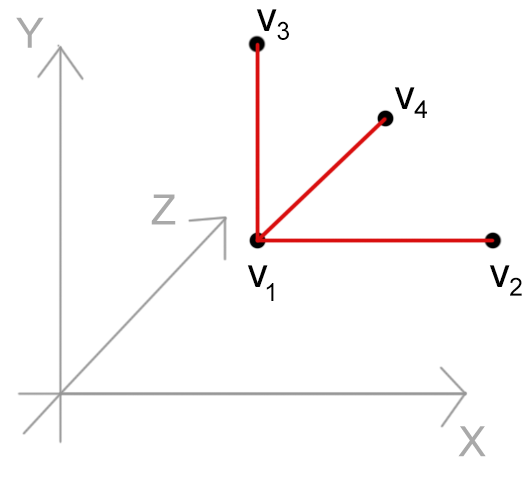
\includegraphics[width=0.35\textwidth]{vertex.png}
	\caption{Vertex with some edges to other vertices}
	\label{fig:vertex}
	\vspace{0.6cm}
\end{wrapfigure}

Quads (quadratic faces) are made of 4 vertices that build the face. Besides the 4 vertices (saved as IDs in the quad class) the quad also needs to know its adjacent quads, its neighbors. To determine what the outside of a face is we need to calculate the normal vector of the face. The normal vector is calculated by the cross product of the quads diagonals (see figure \ref{fig:quad}).

\begin{wrapfigure}{R}{0.45\textwidth}
	\centering
	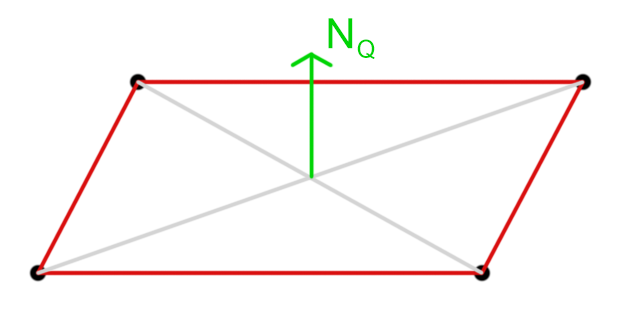
\includegraphics[width=0.4\textwidth]{quad.png}
	\caption{Quad with a normal vector in the center of it}
	\label{fig:quad}
	\vspace{-1cm}
\end{wrapfigure}

For rendering an object it is necessary to read its vertices and faces from a file. For these exercises it can be assumed that all faces are quads. The number of vertices and quads are variable depending on the object that is tried to load in. So instead of using static arrays it is required to use something dynamic like a QVector\footnote{\url{http://doc.qt.io/qt-5/qvector.html}}.

Now the object can be rendered. This will be done in two ways, as quadrilateral polygons to see the faces and how they reflect light (see figure \ref{fig:renderedcube}) and as wireframe to see the vertices and edges.

\begin{wrapfigure}{R}{0.5\textwidth}
	\centering
	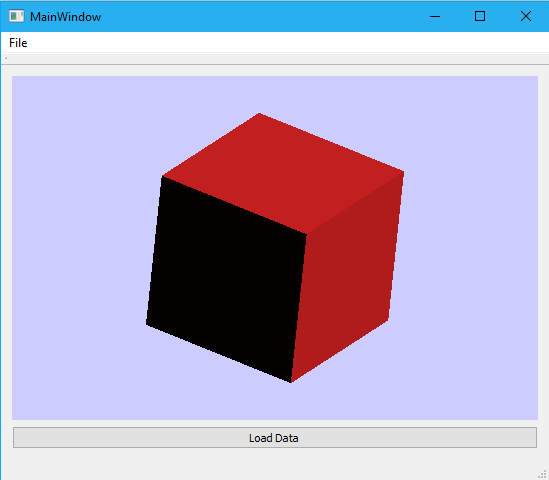
\includegraphics[width=0.45\textwidth]{renderedcube.png}
	\caption{Render of an example cube}
	\label{fig:renderedcube}
\end{wrapfigure}

\subsection{Problem 2: Mesh Connectivity}

In Problem 1 the created classes got variables like valence for the vertices or neighbors of the quads. These need to be calculated now.

The valence of each vertex can be calculated by looking at every quad and see which vertex is next to the other (see figure \ref{fig:faces}) and see with how many other vertices that current vertex is connected. To prevent adding an edge twice to a vertex this needs to be checked as well.

\begin{wrapfigure}{L}{0.5\textwidth}
	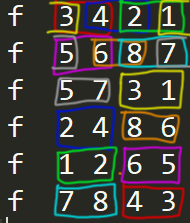
\includegraphics[width=0.45\textwidth]{faces.png}
	\caption{A list of faces from the example cube.obj with edge building vertices shown (first two rows)}
	\label{fig:faces}
\end{wrapfigure}

\begin{wrapfigure}{L}{0.5\textwidth}
	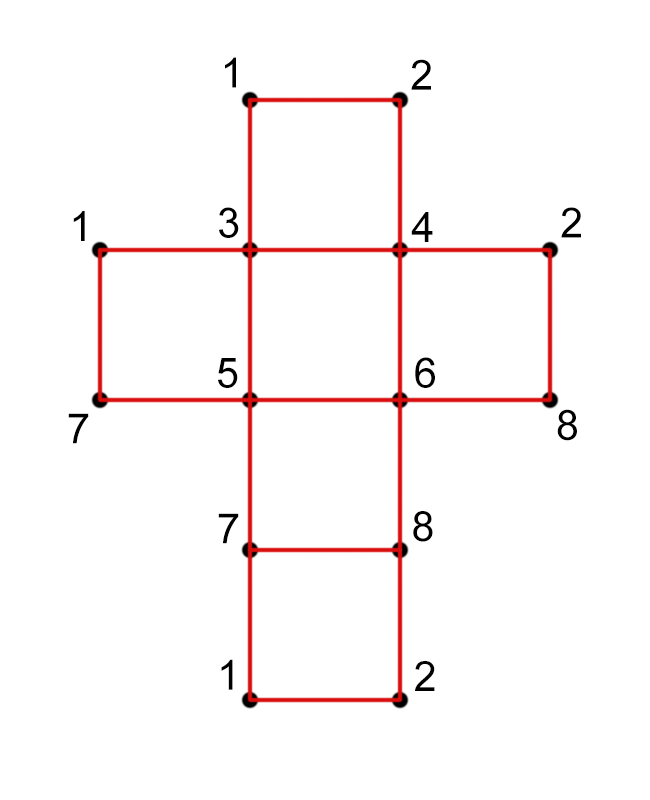
\includegraphics[width=0.45\textwidth]{cube.png}
	\caption{An opened cube with all vertex indices}
	\label{fig:cube}
\end{wrapfigure}

For the neighbors of a quad it needs to be checked if a quad shares the same 2 vertices or edge with another quad, if it does it will be added to the current quad as its neighbor.

\section{Exercise 2: Catmull-Clark Subdivision}
The goal of this exercise is to smooth objects, making them rounder by looking at nearby vertices of the altering vertex.

\subsection{Problem 1: Catmull-Clark Subdivision Masks}
For creating the subdivision mask there are some preparations needed before applying the subdivision in the end.

\subsubsection{Part a: Quad midpoints}
The first and easiest part is the calculation of the midpoints of the quads. To get the midpoint of a quad the average of all vertices of that quad is needed (see equation \ref{eq:face_midpoint}).
\begin{equation} \label{eq:face_midpoint}
        f \ = \overline{v_{f}}
\end{equation} 
So for quads every vertex needs to be devided by 4.

\subsubsection{Part b: Edge midpoints}
The next thing needed for the subdivision mask are midpoints of every edge of an object. So for this kind of midpoint the average of both vertices of that edge and the average of the two quad midpoints next to the edge are needed.
\begin{equation} \label{eq:edge_midpoint}
        e \ = \frac{1}{2} ( \overline{v_{e}} + \overline{f_{e}} )
\end{equation} 
Because two averages of vertices were summed up, this sum needs to divide by two (see equation \ref{eq:edge_midpoint}).

When going through all edges it needs to be prevented that an edge midpoint gets calculated twice due to indices may be flipped in another quad. For example q1 has vertices 1 2 3 4 and q2 has vertices 2 1 5 6, the 1 and 2 are in both quads but in the second one it is the other way around and may not be detected as the same edge.

\subsubsection{Part c: Alternative vertex mask}
Now to get the alternative mask, the alternative vertices are needed. These are calculated as seen in equation \ref{eq:alternative_vertex_mask}.
\begin{equation} \label{eq:alternative_vertex_mask}
        v_{new} \ = \frac{1}{n_{v}} ( 4 \overline{e_{v}} - \overline{f_{v}} + (n_{v}-3) v)
\end{equation} 
$n_{v}$ is the valence of the current vertex, $\overline{e_{v}}$ and $\overline{f_{v}}$ are the averages of all edge and face midpoints next to the vertex and $v$ the original vertex.

After the alternative vertices are calculated they will replace the old originals.

\subsection{Problem 2: Recursive Subdivision}
At the end all new vertices (face and edge midpoints and alternative vertices) get connected to new sub-faces, overwriting the old faces to restore the mesh connectivity. When the subdivision gets applied multiple times, the object gets more and more smoothed.


\end{document}
